\section{PermLLM框架}
经过前文的梳理和分析,我们可以看到拆分学习应用于大模型的隐私推断存在严重的隐私泄漏问题,与此同时,密码学方法则存在着严重的计算通讯开销问题。
%
我们注意到,密码学在进行大模型隐私推断时,其主要的开销也在于非线性激活函数GeLU上。
由于GeLU的非线性较强,各种密码学方案往往采用高阶多项式对其进行拟合,从而带来了严重的计算开销。
%
现有研究的分析表明,GeLU、层归一化等的通讯开销甚至可以达到线性计算(矩阵乘法等)的一百多倍。
%
因此,优化基于密码学的大模型隐私推断的关键在于优化非线性函数。
%
%

而上一章提出的基于秘密分享和随机排列的安全神经网络框架正是对神经网络的非线性激活函数进行优化,极大提高了神经网络隐私推断和训练的效率,同时尽可能地维持了安全性。
%
在此基础上,本章我们对此针对大模型进行进一步优化,提出融合密码学方法和随机排列的基础上,实现高效安全的大模型隐私推断框架PermLLM。
%
PermLLM框架面向的场景为两方推断的场景,且存在一个辅助第三方用于离线计算。
%
$P_0$为模型拥有方(如OpenAI),其拥有模型的所有参数信息。
%
$P_1$为用户,其目标是获取大模型的关于自身的文本输入的回复。
%
$P_2$为辅助第三方,其参与离线计算阶段,用于生成安全乘法和安全排列的预计算值。
%
我们采用了半可信的安全性设定,同\autoref{}一致。


我们将大语言模型的计算分为三个部分:线性部分、非线性部分和下标选择阶段。
其中线性阶段包含了线性层、注意力分数计算、层归一化后的逐元素线性映射等;
非线性阶段包含了GeLU激活函数、注意力分数的Softmax计算、层归一化的计算等;
而下标选择阶段则是根据预测的分数安全地产生预测词语的下标的阶段。
%
对于线性阶段,我们通过改进的秘密分享协议进行高效计算;
对于非线性阶段,我们采用基于安全随机排列协议的逐元素计算协议进行计算;
对于下标选择阶段,我们基于随机排列和同态加密设计了安全的下标选择协议,不仅支持常用的选取最大分数的词语,也支持按照概率采样等复杂的下标选择策略。
%


\subsection{隐私推断的三个阶段}
许多基于秘密分享技术的隐私保护机器学习框架会按照两个阶段运行,分别是离线(Offline)阶段和在线(Online)阶段。
%
考虑$P_0$和$P_1$要安全地计算$f(X)$的情况,其中$X$被秘密分享在两方之间,而$f$则是一个固定的函数。
%
在离线阶段,$X$还未出现,$P_0$和$P_1$并不需要知道$X$的具体值。
%
但是其可以对未来的$f(X)$进行一些准备工作,比如生成Beaver三元组来辅助安全乘法计算。
%
在在线阶段,$P_0$和$P_1$得到了$X$的具体值,再进行后续的工作。
%t
通过这种方法,参与方可以在还未进行具体的隐私计算任务时提前准备,从而可以减少具体输入出现后的安全计算的开销。

%
而在PermLLM中,我们采用类似的思想,将隐私推断分为三个阶段,分别是初始化阶段、离线阶段、在线阶段。
%
其中初始化阶段和对应的大模型权重有关,在大模型权重不改变的情况下,初始化阶段仅需执行一次。
%
离线阶段和在线阶段则和一般隐私保护机器学习框架中的定义相同。
每一次离线阶段会产生一些预计算值供在线阶段使用,而每一次在线阶段都会消耗一次离线阶段产生的预计算值。
%
比如,一个可能的运行序列可以是“初始化-离线-在线-离线-在线”,
也可以是“初始化-离线-离线-在线-在线”。
但是“初始化-离线-在线-在线-离线”是一个不合法的顺序,因为第二个在线阶段时已经没有预训练的值供其使用。

\subsection{优化的秘密分享乘法}


\subsubsection{针对线性层的秘密分享乘法}
我们首先考虑大预言模型中的线性层。
%
线性层的计算可以表示为$W \bvec x + \bvec b$,其中$W \in \mathbb R^{d\times d}$是一个大矩阵,表示权重;$\bvec x \in \mathbb R^{d}$则是输入文本相关的隐层表征。
%
在秘密分享中,共有两次通讯,分别是离线时$P_2$分发Beaver三元组($U\bvec v = \bvec w$)给$P_0$和$P_1$,和在线时$P_0$和$P_1$恢复出$W - U$和$\bvec x - \bvec v$。
%
我们注意到,由于大模型推断过程中权重$W$是固定不变的,我们可以产生一次Beaver三元组中的$U$,同时$W - U$也只需恢复一次。
因此我们可以把这些计算安排到初始化阶段进行。
%
而输入相关的$\bvec x$则会每次变化,因此三元组中的$\bvec v$和对应的$\bvec w=U\bvec v$会被每一次在线运算阶段消耗,需要在每次离线阶段重新生成。
%
因为$W$的大小是$\bvec x$的$d$倍(在大语言模型中$d > 10^3$),因此将有关$W$的计算提前到初始化阶段单次计算,可以极大地减少在线阶段和离线阶段的通讯开销。


我们在\autoref{alg:perm-llm:secure_mul_fixed}中具体描述上述算法。
同时,在\autoref{fig:perm-llm:ssmul}中,我们也对比了原始的秘密分享乘法和优化的$X$固定的秘密分享乘法。
%
利用$X$是$P_0$已知的特性,我们可以把$P_0$计算的$(X-U)(Y-V) + \langle U \rangle_0(Y-V)$,以及$P_1$计算的$\langle U \rangle_1(Y-V)$合并,
变成仅需$P_0$计算$X(Y-V)$。
%
此时$P_1$无需知道$Y-V$,只需将自身的$\langle Y \rangle_1 - \langle V \rangle_1$发送给$P_0$即可。
因此我们进一步将在线阶段的通讯次数从2轮减少到1轮。
%


\begin{algorithm}[h!]
    \caption{安全常数乘法\textsf{SecureMul}$_F(X, Y)$}
    \label{alg:perm-llm:secure_mul_fixed}
    \begin{algorithmic}[1]
    \Require $P_0$ 持有常数 $X$. 秘密分享的输入 $\langle Y \rangle$
    
    \Ensure 秘密分享的乘积 $\langle Z \rangle = \langle XY \rangle$
    
    \item[\underline{初始化阶段:}]
    %
    \State $P_2$ 产生随机的 $U$ (和 $X$ 形状相同) 并发送给 $P_0$
    %
    \State $P_0$ 发送 $X - U$ 给 $P_1$
    
    \item[\underline{离线阶段:}]
    \State $P_2$ 产生随机的 $V$ (和$Y$ 形状相同), 并且分享 $V, W \gets UV$ 给 $P_0$ 和 $P_1$
    
    \item[\underline{在线阶段:}]
    \State $P_1$ 发送 $\langle Y \rangle_1 - \langle V \rangle_1$ 给 $P_1$,$P_1$ 恢复 $X - U$
    %
    \State $P_0$ 计算 $\langle Z \rangle_0 \gets X(Y-V) + (X-U)\langle V \rangle_0 + \langle W \rangle_0$
    %
    \State $P_1$ 计算 $\langle Z \rangle_1 \gets (X-U) \langle V \rangle_1 + \langle W \rangle_1$
    \end{algorithmic}
\end{algorithm}


\begin{figure}[h!]
    \centering
    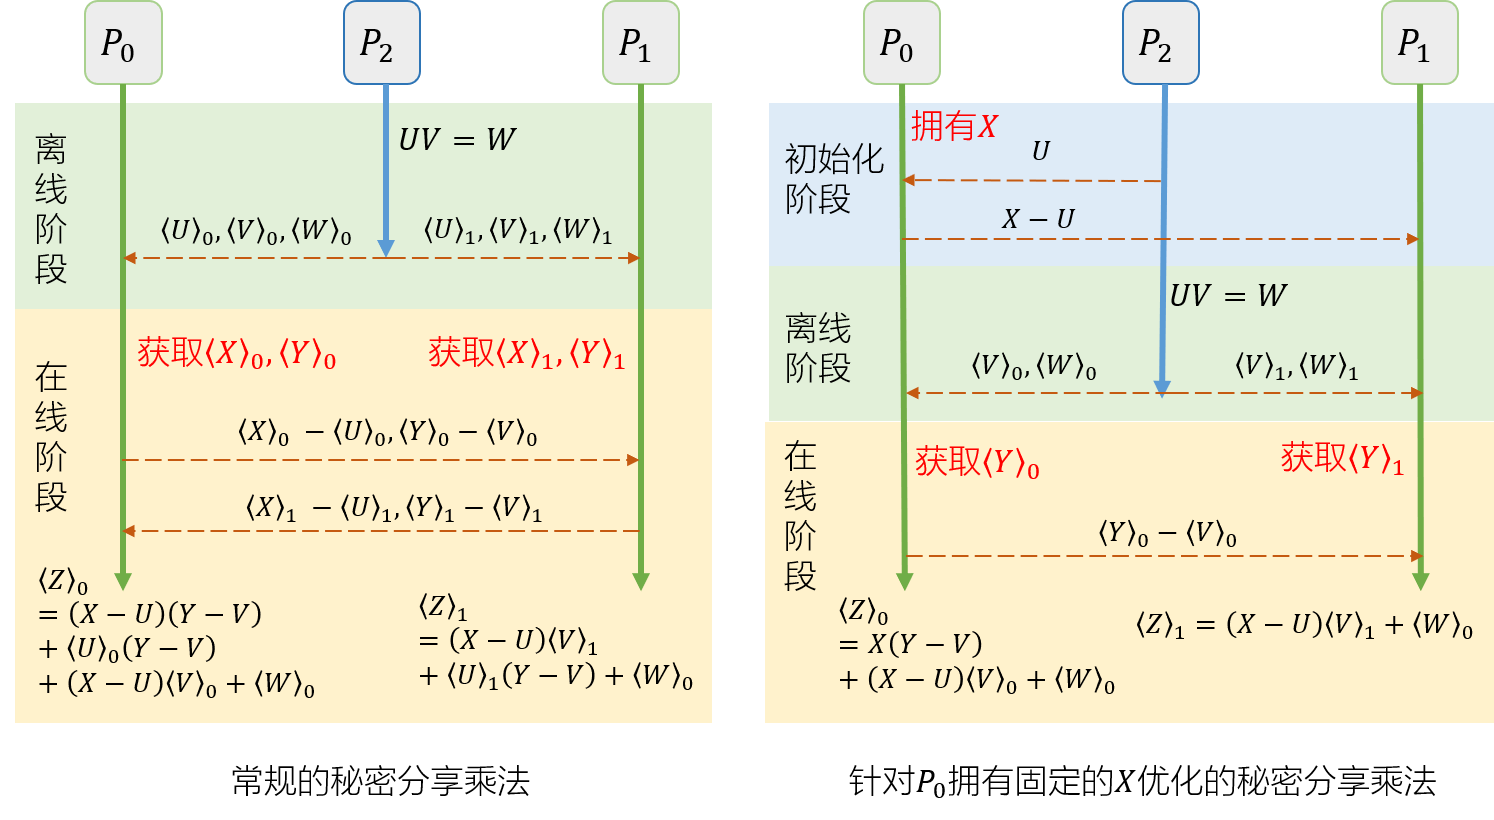
\includegraphics[width=\linewidth]{Z_Resources/perm-llm_ssmul.png}    
    \caption{优化的秘密分享乘法与原始秘密分享乘法的对比}
    \label{fig:perm-llm:ssmul}
\end{figure}


\subsubsection{针对注意力的秘密分享乘法}
在计算注意力分数时,我们需要将当前的查询向量 $\bvec q_i$ 与多个键向量 $\bvec k_1, \cdots, k_n$ 求内积,且注意到在单次文本生成任务中,每轮都会有一个新的键向量加入。
%
如果把键向量构成的矩阵当作$X$,我们可以发现情况与线性层有所类似。
乘数$X$虽然不是固定的,但是其每一轮只会加入一个新的向量,而其余部分保持不变。
%
因此,我们可以借用针对线性层优化的安全秘密分享乘法中的思想,在每一轮在线阶段的运算中,只考虑 $X$ 新增加的部分(此处记作$X'$)恢复出 $X' - U'$,从而更新原有的 $X - U$上。
%